%%%%%%%%%%%%%%%%%%%%%%%%%%%%%%%%%%%%%%%%%%%%%%%%%%%%%%%%%%%%%%%
%
% Welcome to Overleaf --- just edit your LaTeX on the left,
% and we'll compile it for you on the right. If you open the
% 'Share' menu, you can invite other users to edit at the same
% time. See www.overleaf.com/learn for more info. Enjoy!
%
%%%%%%%%%%%%%%%%%%%%%%%%%%%%%%%%%%%%%%%%%%%%%%%%%%%%%%%%%%%%%%%


% Inbuilt themes in beamer
\documentclass{beamer}

% Theme choice:
\usetheme{CambridgeUS}

% Packages
\usepackage{graphicx}
\graphicspath{{images/}}
\usepackage{gensymb}
\usepackage{amssymb}
\usepackage[cmex10]{amsmath}
\usepackage{amsthm}
\usepackage[export]{adjustbox}
\usepackage{bm}
\usepackage{longtable}
\usepackage{enumitem}
\usepackage{mathtools}
 \usepackage{tikz}
\usepackage[breaklinks=true]{hyperref}
\usepackage{listings}
\usepackage{color}                                            %%
\usepackage{array}                                            %%
\usepackage{longtable}                                        %%
\usepackage{calc}                                             %%
\usepackage{multirow}                                         %%
\usepackage{hhline}                                           %%
\usepackage{ifthen}                                           %%
\usepackage{lscape}     
\usepackage{multicol}
\usepackage{enumerate}
\DeclareMathOperator*{\Res}{Res}
\renewcommand\thesection{\arabic{section}}
\renewcommand\thesubsection{\thesection.\arabic{subsection}}
\renewcommand\thesubsubsection{\thesubsection.\arabic{subsubsection}}
\renewcommand\thesectiondis{\arabic{section}}
\renewcommand\thesubsectiondis{\thesectiondis.\arabic{subsection}}
\renewcommand\thesubsubsectiondis{\thesubsectiondis.\arabic{subsubsection}}
\hyphenation{op-tical net-works semi-conduc-tor}
\def\inputGnumericTable{}                                 %%
\lstset{
frame=single, 
breaklines=true,
columns=fullflexible
}

\newcommand{\BEQA}{\begin{eqnarray}}
\newcommand{\EEQA}{\end{eqnarray}}
\newcommand{\define}{\stackrel{\triangle}{=}}
\newcommand*\circled[1]{\tikz[baseline=(char.base)]{
    \node[shape=circle,draw,inner sep=2pt] (char) {#1};}}
%\bibliographystyle{IEEEtran}
\providecommand{\mbf}{\mathbf}
\providecommand{\pr}[1]{\ensuremath{\Pr\left(#1\right)}}
\providecommand{\qfunc}[1]{\ensuremath{Q\left(#1\right)}}
\providecommand{\sbrak}[1]{\ensuremath{{}\left[#1\right]}}
\providecommand{\lsbrak}[1]{\ensuremath{{}\left[#1\right.}}
\providecommand{\rsbrak}[1]{\ensuremath{{}\left.#1\right]}}
\providecommand{\brak}[1]{\ensuremath{\left(#1\right)}}
\providecommand{\lbrak}[1]{\ensuremath{\left(#1\right.}}
\providecommand{\rbrak}[1]{\ensuremath{\left.#1\right)}}
\providecommand{\cbrak}[1]{\ensuremath{\left\{#1\right\}}}
\providecommand{\lcbrak}[1]{\ensuremath{\left\{#1\right.}}
\providecommand{\rcbrak}[1]{\ensuremath{\left.#1\right\}}}
\theoremstyle{remark}
\newtheorem{rem}{Remark}
\newcommand{\sgn}{\mathop{\mathrm{sgn}}}
%\providecommand{\abs}[1]{\left\vert#1\right\vert}
%\providecommand{\res}[1]{\Res\displaylimits_{#1}} 
%\providecommand{\norm}[1]{\left\lVert#1\right\rVert}
%\providecommand{\norm}[1]{\lVert#1\rVert}
%\providecommand{\mtx}[1]{\mathbf{#1}}
%\providecommand{\mean}[1]{E\left[ #1 \right]}
\providecommand{\fourier}{\overset{\mathcal{F}}{ \rightleftharpoons}}
%\providecommand{\hilbert}{\overset{\mathcal{H}}{ \rightleftharpoons}}
\providecommand{\system}{\overset{\mathcal{H}}{ \longleftrightarrow}}
	%\newcommand{\solution}[2]{\textbf{Solution:}{#1}}
\newcommand{\solution}{\noindent \textbf{Solution: }}
\newcommand{\cosec}{\,\text{cosec}\,}
\providecommand{\dec}[2]{\ensuremath{\overset{#1}{\underset{#2}{\gtrless}}}}
\newcommand{\myvec}[1]{\ensuremath{\begin{pmatrix}#1\end{pmatrix}}}
\newcommand{\mydet}[1]{\ensuremath{\begin{vmatrix}#1\end{vmatrix}}}
\newcommand*{\permcomb}[4][0mu]{{{}^{#3}\mkern#1#2_{#4}}}
\newcommand*{\perm}[1][-3mu]{\permcomb[#1]{P}}
\newcommand*{\comb}[1][-1mu]{\permcomb[#1]{C}}
\numberwithin{equation}{subsection}
\makeatletter
\@addtoreset{figure}{problem}
\makeatother
\let\StandardTheFigure\thefigure
\let\vec\mathbf
\renewcommand{\thefigure}{\theproblem}
\def\putbox#1#2#3{\makebox[0in][l]{\makebox[#1][l]{}\raisebox{\baselineskip}[0in][0in]{\raisebox{#2}[0in][0in]{#3}}}}
     \def\rightbox#1{\makebox[0in][r]{#1}}
     \def\centbox#1{\makebox[0in]{#1}}
     \def\topbox#1{\raisebox{-\baselineskip}[0in][0in]{#1}}
     \def\midbox#1{\raisebox{-0.5\baselineskip}[0in][0in]{#1}}
\vspace{3cm}


% Title page details: 
\title{Assignment 8} 
\author{Hema Sri Cheekatla, CS21BTECH11013}
\date{\today}
\logo{\large \LaTeX{}}


\begin{document}
% Title page frame
\begin{frame}
    \titlepage 
\end{frame}

% Remove logo from the next slides
\logo{}


% Outline frame
\begin{frame}{Outline}
    \tableofcontents
\end{frame}

% Question frame
\begin{frame}{Question}
    \section{Question}
    The random variables x and y are independent with,\newline
    \begin{align}
        f_x &=  \frac{x}{\alpha^2}e^{\frac{-x^2}{2\alpha^2}}U(x) \\
        f_y &= \begin{cases} \frac{1}{\pi \sqrt{1 - y^2}} &, |y| < 1 \\
            0 &, |y| > 1 \end{cases} 
    \end{align}
    Show that the random variable z=xy is $N(0, \alpha^2)$
\end{frame}

% Solution frames
\begin{frame}{Solution}
    \section{Solution}
    we have z=xy and if we assume x = w, then y = z/w \newline
    Now their respective regions are as follows
    \begin{figure}
        \centering
        \begin{subfigure}{\textwidth}
            \centering
            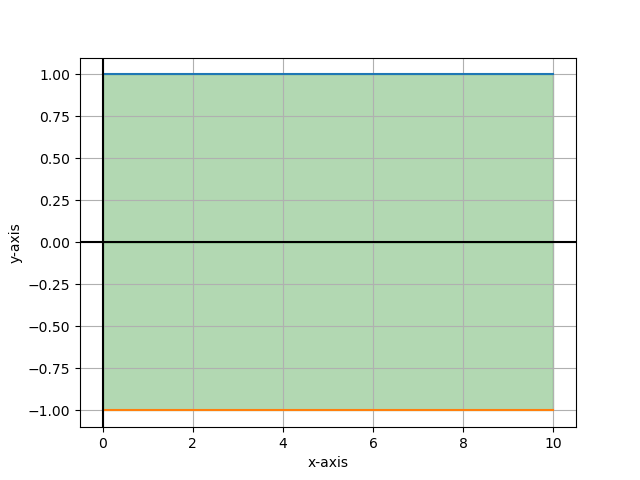
\includegraphics[width=0.4\linewidth]{Graph}
         %   \caption{$x>0$ and $|y| < 1$}
            \label{fig:sub1}
        \end{subfigure}%
    \begin{subfigure}{\textwidth}
        \centering
        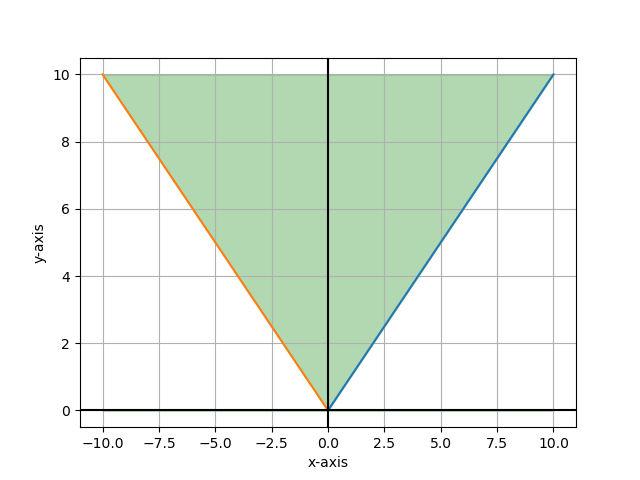
\includegraphics[width=0.4\linewidth]{Graph2}
%        \caption{x = w and y = z/w}
        \label{fig:sub2}
    \end{subfigure}
   % \caption{A figure with two subfigures}
    \label{fig:test}
\end{figure}
$x>0$ and $|y| < 1$ and x = w and y = z/w
\end{frame}

\begin{frame}{Solution}
    since y = z/w,
    \begin{align}
        f_{wz}(w, z) &= \frac{1}{|x|}f_{xy}(x, y) \\
        f_{wz}(w, z) &= \frac{1}{x} \frac{x}{\alpha^2}e^{\frac{-x^2}{2\alpha^2}} \frac{1}{\pi \sqrt{1 - y^2}} \\
        \implies f_{wz}(w, z) &= \frac{1}{\pi \alpha^2}\frac{e^{\frac{-w^2}{2\alpha^2}}}{\pi \sqrt{1 - \frac{z^2}{w^2}}}
    \end{align}
\end{frame}

\begin{frame}{Solution}
    \begin{align}
        f_z(z) = \frac{1}{\pi \alpha^2}\int_{|w|}^{\infty} \frac{e^{\frac{-w^2}{2\alpha^2}}}{\sqrt{w^2 - z^2}} w \,dw 
    \end{align}
    Assume, 
    \begin{align}
        \sqrt{w^2 - z^2} &= t \\
        \frac{2w \,dw}{2\sqrt{w^2 - z^2}} &= \, dt \\
        \implies w \, dw &= t\, dt
    \end{align}
\end{frame}

\begin{frame}{Solution}
    \begin{align}
       \implies f_z(z) &= \frac{1}{\pi \alpha^2} \int_{0}^{\infty} \frac{e^{\frac{-(t^2 + z^2)}{2\alpha^2}}}{t} t \, dt \\
       &= \frac{1}{\pi \alpha^2} e^{\frac{-z^2}{2\alpha^2}}\int_{0}^{\infty} e^{-(\frac{t}{\sqrt{2\alpha^2}})^2} \, dt \\
       \text{Let } \frac{t}{\sqrt{2\alpha^2}} &= k  \\
       \implies \, dt &= \sqrt{2\alpha^2} \, dk \\
       \text{Hence } f_z(z) &= \frac{1}{\pi \alpha^2} e^{\frac{-z^2}{2\alpha^2}}\sqrt{2\alpha^2} \int_{0}^{\infty} e^{-k^2} \, dk 
    \end{align}
\end{frame}

\begin{frame}{Solution}
    From the known result of 
    \begin{align}
        \int_{-\infty}^{\infty} e^{-x^2} \, dx &= \sqrt{\pi} \\
        \implies f_z(z) &= \frac{1}{\pi \alpha^2}e^{\frac{-z^2}{2\alpha^2}} \sqrt{2\alpha^2} \frac{\sqrt{\pi}}{2}  \\
       f_z(z) &= \frac{1}{\sqrt{2\pi\alpha^2}}e^{\frac{-z^2}{2\alpha^2}}
    \end{align}
    Hence the random variable $z = xy$ is $N(0,\alpha^2)$
\end{frame}
\end{document}